\documentclass[a4paper,11pt, oneside]{book}
\usepackage[utf8]{inputenc}
\usepackage[francais]{babel}
\usepackage[T1]{fontenc}
\usepackage{graphicx}
\usepackage{float}
\usepackage{wrapfig}
\usepackage{setspace}
\usepackage{geometry}
\usepackage{multicol}
\usepackage{etoolbox}
\usepackage{color}
\usepackage[explicit,pagestyles]{titlesec}
\usepackage[absolute,overlay]{textpos}
\usepackage{fancyhdr}
\usepackage{fontspec}
\usepackage{eurosym}
\usepackage{titlesec}


% ====== CONFIG ========
\setmainfont{Roboto}
\setsansfont{Roboto}
\setmonofont{Roboto}
\newfontfamily\light{Roboto Slab Light}
\graphicspath{{img/}}
\setlength{\unitlength}{1mm}

\makeatletter

\definecolor{primary}{RGB}{229, 45, 39}

\fancypagestyle{plain}{
	\fancyhf{}
	\fancyhead[R]{\thepage}
	\renewcommand{\headrulewidth}{0pt}
	\renewcommand{\footrulewidth}{0pt}
	\renewcommand{\chaptermark}[1]{\markboth{\ }{}}
}


\titleformat{\chapter}[display]
	{\huge\light\color{primary}}{#1}{0pt}{\Huge}
\titlespacing{\chapter}
	{0pt}{0pt}{0pt}

\titleformat{\section}
	{\large\color{primary}}{\thesection}{0pt}{\MakeUppercase{#1}}
%\titlespacing*{\section}{0pt}{2\baselineskip}{0pt}


\setlength{\TPHorizModule}{1mm}
\setlength{\TPVertModule}{1mm}
\def\sizeMedia{38}
\def\size{8cm}
\def\sizeMargin{0.2cm}
\def\margin{2}
\def\fixMargin{0}

\pagestyle{plain}


\title{Compte rendu d'activité}
\author{Yann Prono}
\date{\today}

\def\school{TELECOM Nancy}
\def\schoolAddress{193 Avenue Paul Muller}
\def\schoolPostalCode{54602}
\def\schoolCity{Villers-lès-Nancy}
\def\schoolCodeAndCity{\schoolPostalCode, \schoolCity}
\def\schoolYear{2016 - 2017}

\def\club{Club Studio}
\def\chair{Eliot GODARD}
\def\secretary{Yann PRONO}
\def\banker{Ansel GAMET}
\def\teacher{Isabelle HEUDIARD}
\def\bde{Victor CHOLLEY-BARROYER}

\def\schoolYear{2015 - 2016}

% ====== END CONFIG ========


\begin{document}

	\begin{titlepage}
		\thispagestyle{empty}


\begin{flushleft}
\school\\
\schoolAddress\\
\schoolCodeAndCity\\
Université de Lorraine\\
\end{flushleft}

\vspace{0.6cm}

\begin{center}
\rule{\textwidth}{0.8pt}

\vspace{0.6cm}

\baselineskip=3pt
{\Huge \bfseries{PCD - Coding Week}}\\
\LARGE{Application java interfaçant le système Youtube}\\

\vspace{0.2cm}

\rule{\textwidth}{0.8pt}
\end{center}

\vspace{0.5cm}

	\begin{center}
		
\includegraphics[width=0.8\textwidth]{tn.eps}
	\end{center}

	\vspace{0.5cm}
	\begin{center}
		\Large{Ansel GAMET}\\
		\Large{Eliot GODARD}\\
		\Large{Lucas MARTINEZ}\\
		\Large{Yann PRONO}
	\end{center}

	\vspace{0.5cm}
	\begin{center}
		\Large{\schoolYear}
	\end{center}

\vspace{0.5cm}
	\begin{center}
		
\includegraphics[width=0.3\textwidth]{ul.eps}
	\end{center}
	\end{titlepage}

	\newpage

	\newpage\null\thispagestyle{empty}\newpage
	\setcounter{page}{1}

	\chapter{Lundi}


La première étape de la journée a été de préparer les machines de chaque étudiant (installation des dépendances, javaFX ...).
Cette étape nous a pris un certain temps à cause de petits problèmes techniques.\\

\noindent Nous avons eu ensuite la première réunion de Brigitte wrobel-dautcourt. Elle nous a donné  quelques conseils afin de bien démarrer cette semaine de programmation intensive en fixant les fonctionnalités de l'application. Un brainstorming a permi de lister ces fonctionnalités qui sont au nombre de 12 actuellement:\\

\begin{enumerate}
	\item Chercher une vidéo en utilisant l'API youtube
	\item Afficher la liste des résultats pour une requête utilisateur
	\item Regarder une vidéo youtube online
	\item Pouvoir controler le vidéo player youtube
	\item Pouvoir regarder une vidéo youtube offline
	\item Sauvegarder les vidéos favorites
	\item Créer une playlist de vidéos
	\item Améliorer l'éxperience utilisateur avec des thumbnails avancés
	\item Suggérer des vidéos selon des critères donnés
	\item Proposer une navigation intuitive
	\item Authentifier un utilisateur sur Youtube
	\item Pouvoir commenter ou \textit{liker} une vidéo
	\item Afficher plus d'information concernant une vidéo (titre, description, commentaires ...)\\
\end{enumerate}


\noindent Ce brainstorming a également été l'ocasion de définir les rôles de chacun:\\

\begin{tabular}{lcr}
	Eliot GODARD & \hspace{1cm} & User interface Développeur et testeur qualité \\
	Ansel GAMET & \hspace{1cm} & User interface Développeur et testeur qualité \\
	Lucas MARTINEZ & \hspace{1cm} & Développeur \\
	Yann PRONO & \hspace{1cm} & Chef de projet \\
\end{tabular}

\clearpage
Le planning a été défini de la sorte:\\

\begin{tabular}{|c|c|c|c|c|c|}
	\hline
	 					& Lundi 	& Mardi 	& Mercredi 		& Jeudi 	& Vendredi\\
	 \hline
		Yann / Lucas 	& 1 (9) 	& 3 (6) 	& 6, 8 			& 10 		& 9, 11, 12 et finition\\
		Ansel / Éliot 	& 2 (4) 	& 4, 5 		& 7 (9) 		& 13 		& 9, 11, 12 et finition\\
	\hline
\end{tabular}

Les numéros de fonctionnalités entre parenthèses sont à développer si les autres fonctionnalités importantes sont déjà réalisées.


\begin{center}
	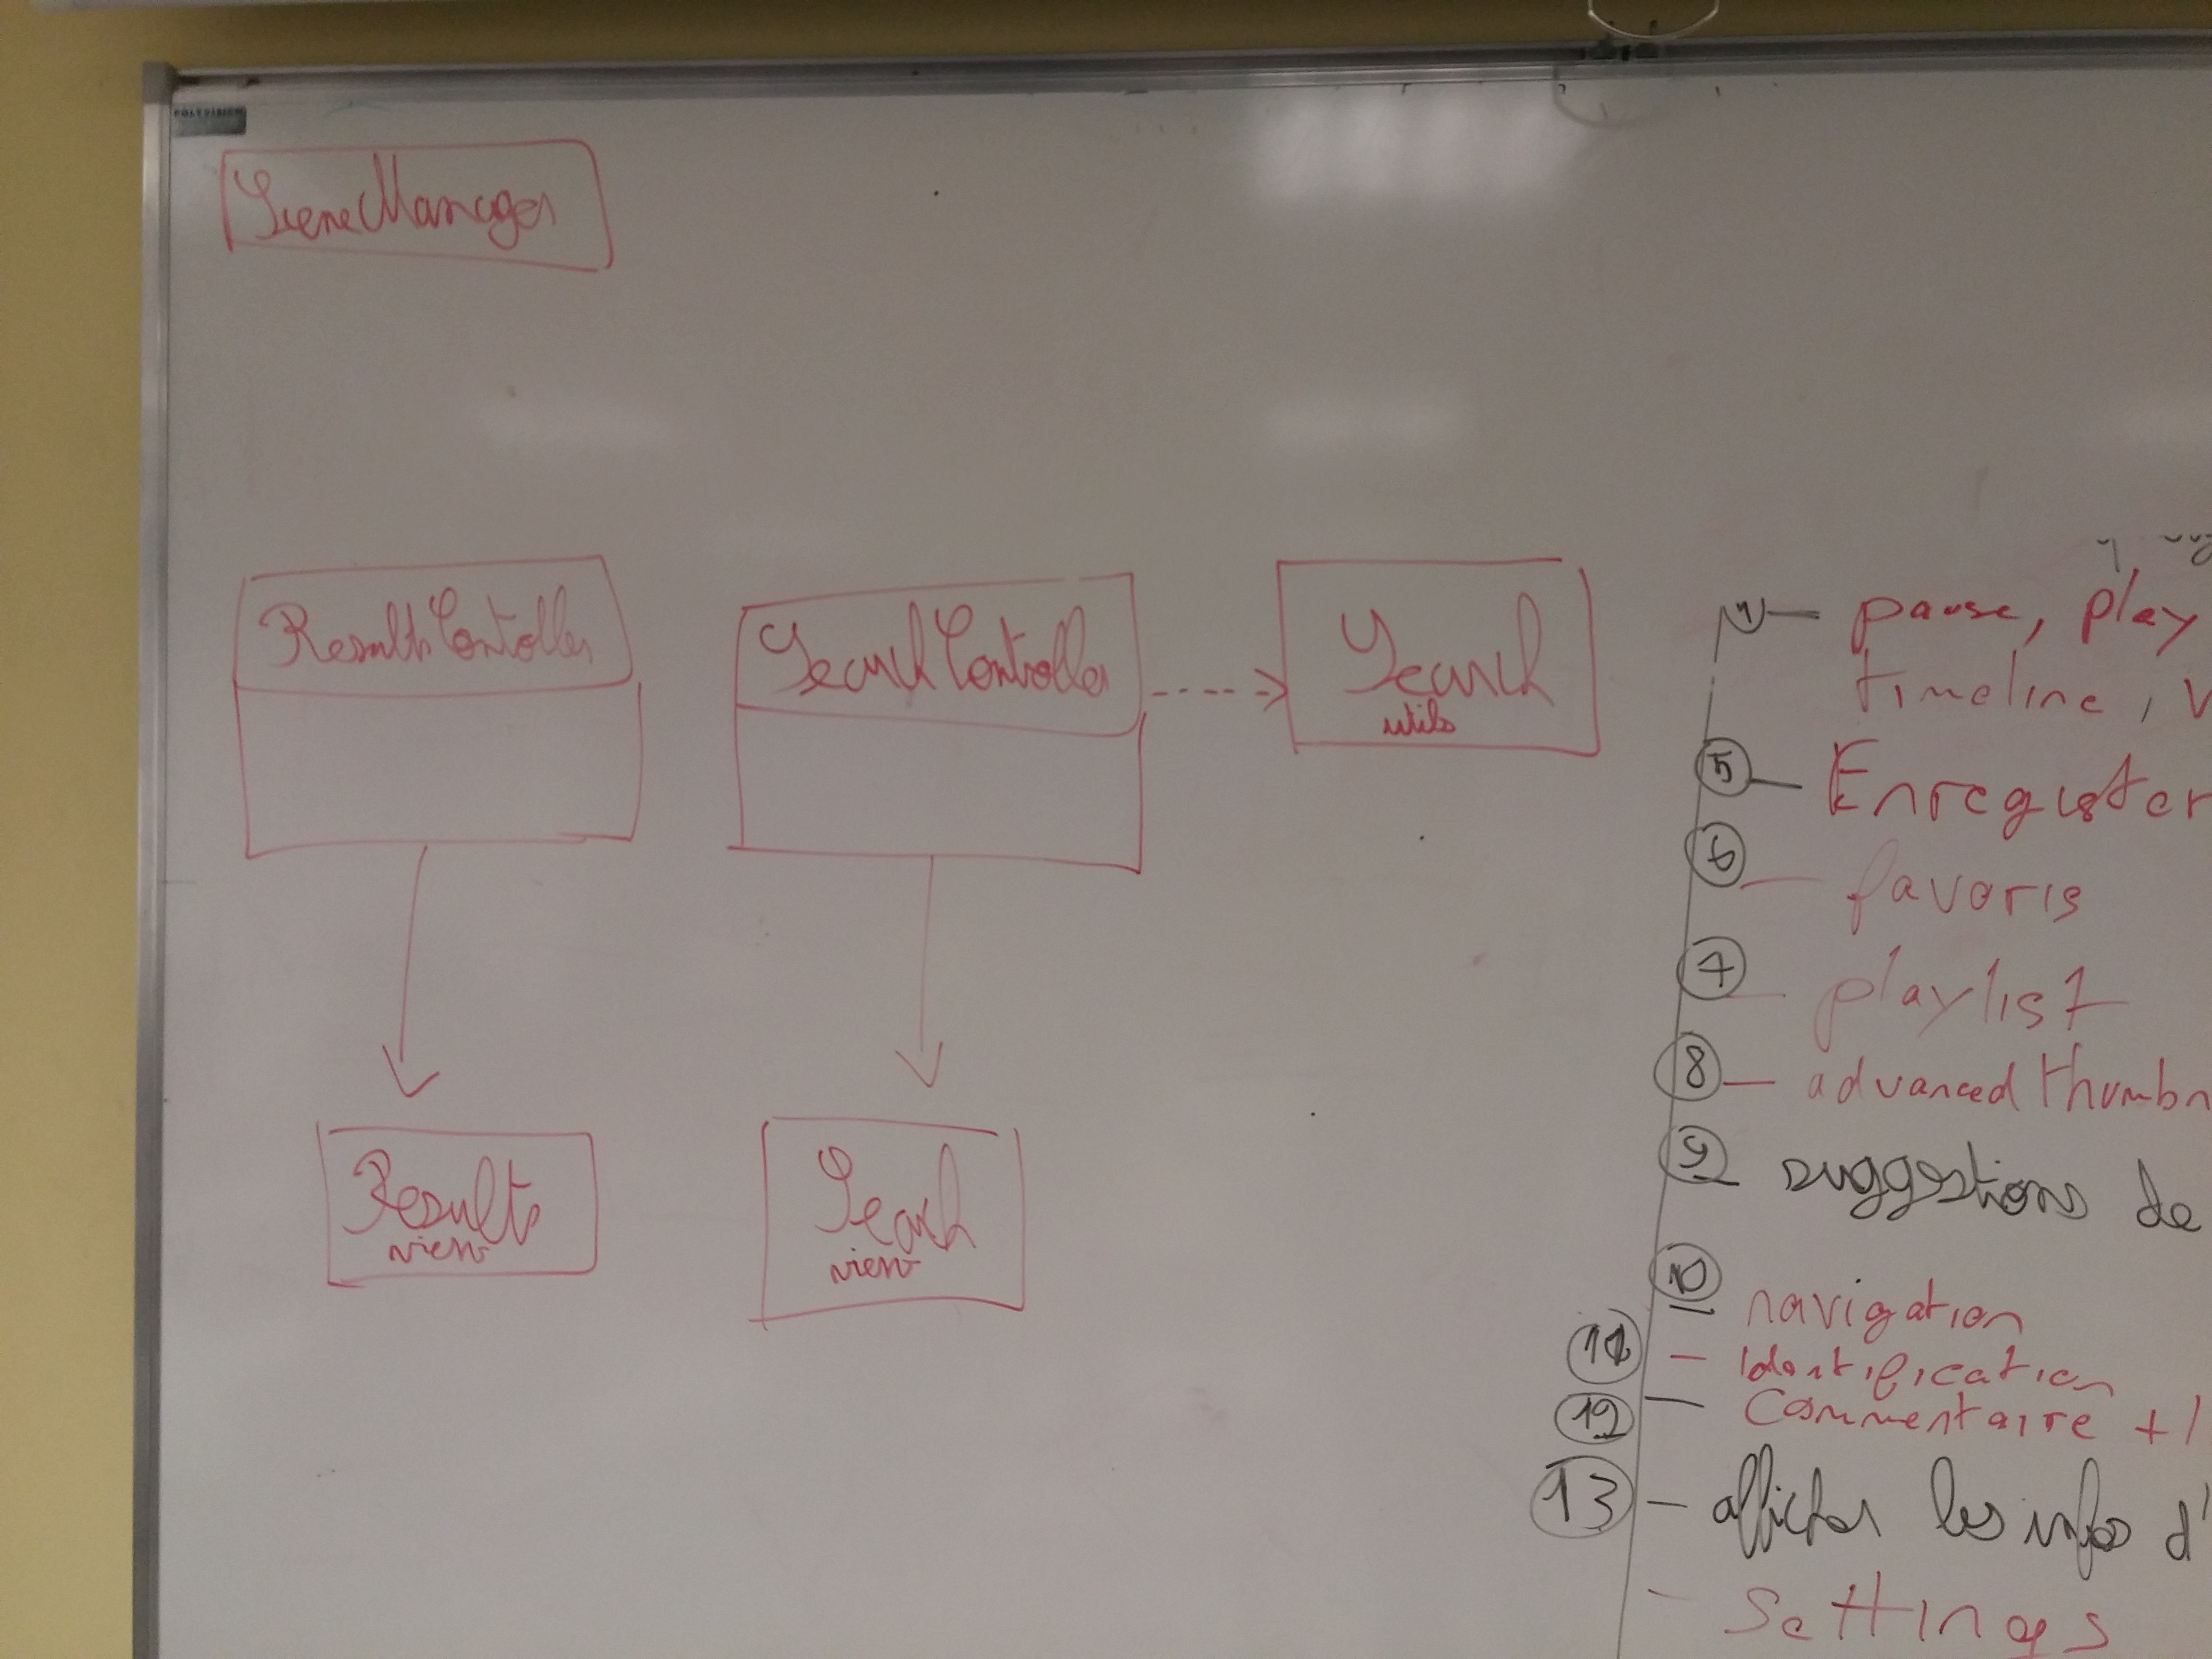
\includegraphics[width=0.8\textwidth]{1.jpg}
\end{center}

À la fin de cette journée, nous avons pu développer la fonctionnalité 1, 2 dans leur majorité. La fonctionnalité 4 est en cours de finition.


\begin{textblock}{0}(20, 190)
	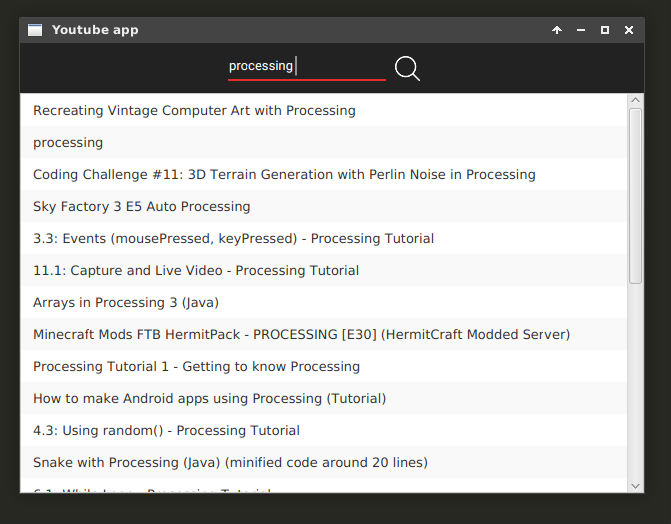
\includegraphics[width=\size, keepaspectratio]{V1.jpg}
\end{textblock}

\begin{textblock}{0}(105, 190)
	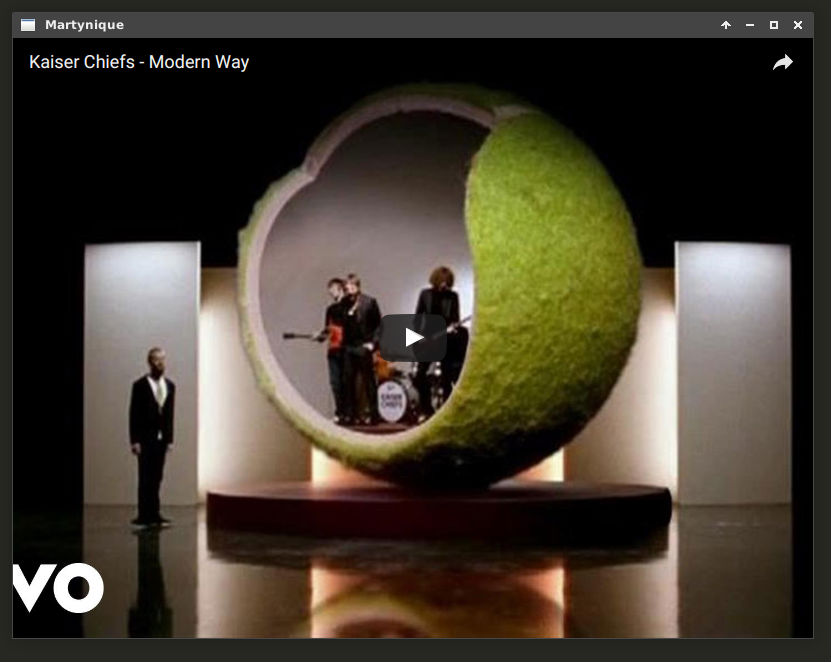
\includegraphics[width=\size]{V1_1.jpg}
\end{textblock}
	\chapter{Mardi}

BUKKAKE \\

\begin{textblock}{0}(20, 190)
	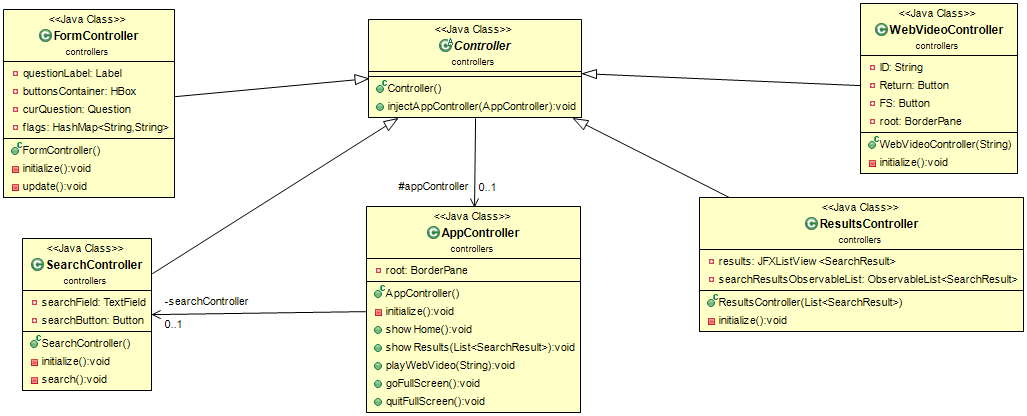
\includegraphics[width=\size, keepaspectratio]{Controllers.jpg}
\end{textblock}

\begin{textblock}{0}(105, 190)
	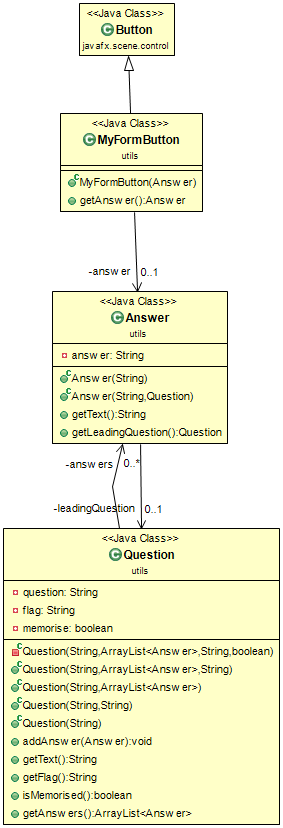
\includegraphics[width=\size]{Form.jpg}
\end{textblock}

\begin{textblock}{0}(20, 190)
	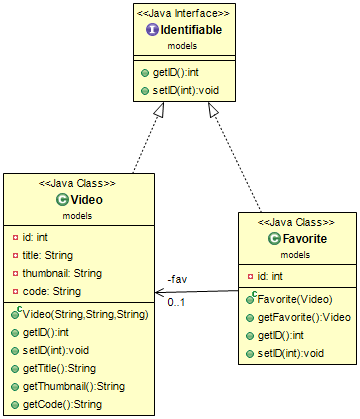
\includegraphics[width=\size, keepaspectratio]{Models.jpg}
\end{textblock}

\begin{textblock}{0}(105, 190)
	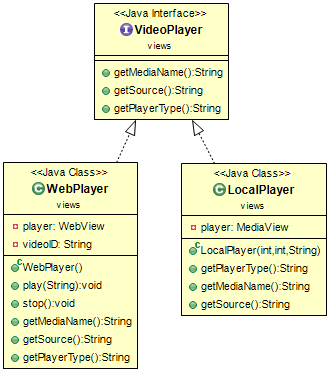
\includegraphics[width=\size]{Players.jpg}
\end{textblock}

\begin{textblock}{0}(105, 190)
	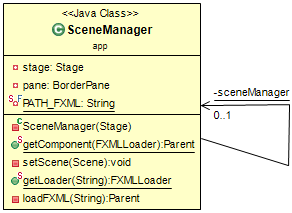
\includegraphics[width=\size]{Autre.jpg}
\end{textblock}
	\chapter{Mercredi}


Les objectifs de cette journée sont les suivants:

\begin{itemize}
	\item Pouvoir regarder un vidéo offline (en retard)
	\item Télécharger une vidéo (en retard)
	\item Sauvegarder des vidéos favoris.
	\item Pouvoir créer une playlist
	\item Améliorer l'éxperience utilisateur avec des thumbnails avancées.
\end{itemize}

La sauvegarde des favoris nous mènent naturellement vers un SGBD. Ce SGBD pourra également nous servir pour le module de suggestion de vidéos.

Nous rencontrons nos premières difficultés pour la conception. Nous commencons à duppliquer du code et des design pattern peuvent être appliqués dans certaines parties du projet. Retravailler la conception du projet nous ferait perdre beaucoup de temps. C'est pourquoi, nous décidons de continuer sur cette voie mais en migrant progressivement vers la nouvelle conception.

Point positif, une avancé importante a été apportée au niveau de l'interface homme-machine. Nous nous inspirons directement de l'application android \textit{Youtube}. De plus, les vidéos favorites de l'utilisateur sont persistés en base de données.


Très grande avancée dans le projet (player design, suggestion, player, base de données, refonte la conception). Le projet est sur une bonne voie

	\clearpage

\end{document}